\section{Exercise 5}
\textit{Recall the superellipsoid movie Chris shown in class... We can define a superellipsoid shape with the 4-vector-norm. For example,$(x^4+y^4+z^4)^\frac{1}{4}=R$ As a practice for the syntax, could you construct three superellipsoid using the above three methods respectively: (a) using "isosurface"; (b) using "poly" or its shortcuts; (c) using"superellipsoid" keyword, what values of $r$, $n$ should you choose? Lastly, consider assigning them different colors and textures! :)}
See \autoref{fig:ex5}.

\begin{figure}[h]
  \centering
  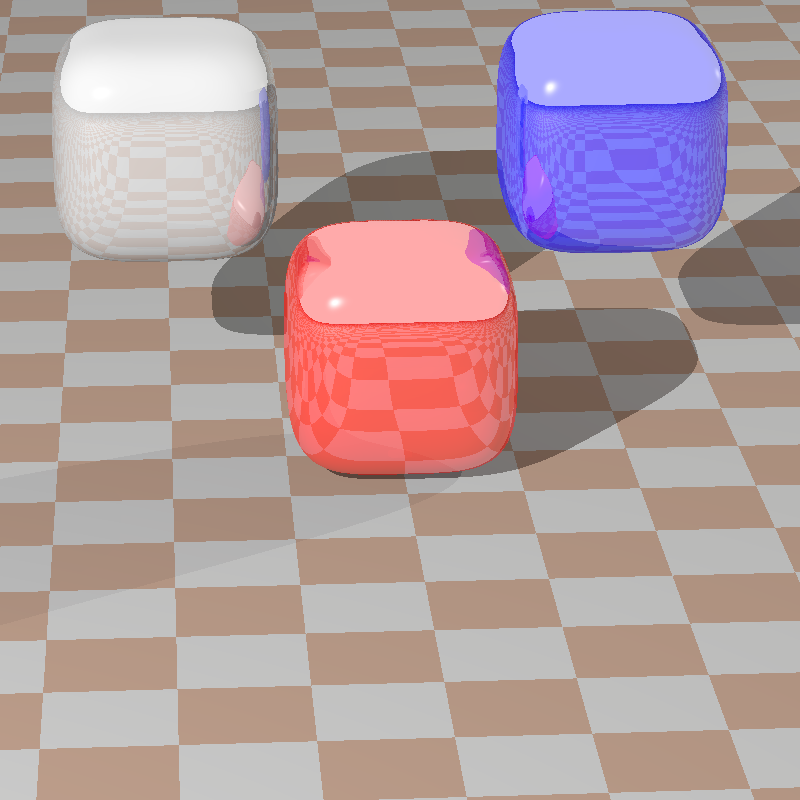
\includegraphics[height=5cm]{ex5.png}
  \caption{Solution for Exercise 5}
  \label{fig:ex5}
\end{figure}